% !TEX program = xelatex
\documentclass[12pt,letterpaper]{article}

% === GEOMETRY (generous margins, roomy) ===
\usepackage[top=1in, bottom=1in, left=1.1in, right=1.1in]{geometry}

% === FONTS ===
% Use explicit OTF filenames so tectonic can pull them from CTAN rather than
% requiring Latin Modern Sans to be installed at the OS font level.
\usepackage{fontspec}
\setmainfont[
  Extension = .otf,
  UprightFont = lmsans10-regular,
  BoldFont = lmsans10-bold,
  ItalicFont = lmsans10-oblique,
  BoldItalicFont = lmsans10-boldoblique,
]{lmsans10}
\setmonofont[
  Extension = .otf,
  UprightFont = lmmono10-regular,
  ItalicFont = lmmono10-italic,
  Scale = 0.85,
]{lmmono10}

\newfontfamily\acbold{ywft-processing-bold}[
  Path=../../system/public/type/webfonts/,
  Extension=.ttf
]

% === PACKAGES ===
\usepackage{xcolor}
\usepackage{enumitem}
\usepackage{tabularx}
\usepackage{fancyhdr}
\usepackage{graphicx}
\usepackage{ragged2e}
\usepackage{microtype}
\usepackage{eso-pic}
\usepackage{tikz}
\usepackage{hyperref}

\graphicspath{{figures/}}

% === COLORS ===
\definecolor{acpink}{RGB}{180,72,135}
\definecolor{acpurple}{RGB}{120,80,180}
\definecolor{acgray}{RGB}{119,119,119}
\definecolor{ruleclr}{RGB}{200,200,200}

% === PALS LOGO (title page only, upright) ===
% Applied via \AddToShipoutPicture* (one-shot, next page only)
% Called just before \begin{document}

% === HYPERREF ===
\hypersetup{
  colorlinks=true,
  linkcolor=acpurple,
  urlcolor=acpurple,
  pdfauthor={Jeffrey Alan Scudder},
  pdftitle={LACMA Art + Technology Lab 2026: Aesthetic Computer},
}

% === HEADER/FOOTER ===
\pagestyle{fancy}
\fancyhf{}
\renewcommand{\headrulewidth}{0pt}
\fancyfoot[C]{\small\color{acgray}\thepage}

% === LISTS ===
\setlist[enumerate]{leftmargin=1.6em, itemsep=0.5em, parsep=0.1em}
\setlist[itemize]{leftmargin=1.4em, itemsep=0.3em}

% === PARAGRAPH ===
\setlength{\parindent}{0em}
\setlength{\parskip}{0.6em}
\RaggedRight

% === HELPERS ===
\newcommand{\ac}{Aesthetic{\color{acpink}.}Computer}
\newcommand{\achead}[1]{%
  \vspace{1.6em}%
  {\color{acpink}\noindent\rule{\textwidth}{1.5pt}}\\[0.4em]
  {\large\bfseries #1}%
  \vspace{0.4em}%
}
\newcommand{\acsubhead}[1]{%
  \vspace{1em}%
  {\color{acgray}\noindent\rule{4cm}{0.5pt}}\\[0.3em]
  {\bfseries #1}%
  \vspace{0.3em}%
}
\newcommand{\cvline}[2]{\noindent\makebox[3.2em][l]{\color{acgray}#1}#2\\[0.15em]}

% ===================================================================
\AddToShipoutPicture*{%
  \begin{tikzpicture}[remember picture, overlay]
    \node[opacity=0.06, anchor=north east]
      at ([xshift=-1.2cm, yshift=-0.8cm]current page.north east)
      {
\includegraphics[width=1.5cm]{pals}};
  \end{tikzpicture}%
}
\begin{document}
\thispagestyle{fancy}

% === TITLE BLOCK ===
\vspace*{0.8em}
\begin{center}
  {\acbold\fontsize{30pt}{34pt}\selectfont Aesthetic{\color{acpink}.}Computer}\\[14pt]
  {\large The Unfinished Instrument}\\[24pt]
  {\color{acgray}\small Jeffrey Alan Scudder}\\[3pt]
  {\color{acgray}\small LACMA Art + Technology Lab · 2026}
\end{center}

\vspace{1.2em}
{\color{acpink}\hrule height 1pt}
\vspace{1em}

{\large\bfseries \ac{} is a bare-metal creative computing system---custom hardware, a handmade programming language, and a social network---that reimagines the personal computer as a live musical instrument for art.}

% =======================================================================
\achead{Project Description}

\ac{} (AC) is a creative computing platform built from first principles. It consists of three interlocking layers: a bare-metal operating system that boots directly into art software, a custom programming language called KidLisp for generative art, and a social network where anyone can publish and share interactive programs called ``pieces.''

The core provocation is simple: what happens when you strip away the consumer operating system---the notifications, the app stores, the surveillance---and build a computer that does nothing but help you make things?

\textbf{AC Native} is our answer in hardware. It is a Linux kernel that boots directly into art software on x86\_64 UEFI laptops, running a custom C runtime as PID\,1---no desktop, no window manager, no browser. The system renders graphics through DRM without a compositor, reads input from raw evdev streams, and synthesizes audio sample-by-sample through ALSA at 192\,kHz with 32-voice polyphony. A built-in \texttt{code} command drops into a native terminal running Anthropic's Claude Code---making AC Native the only bare-metal creative OS we know of with an AI coding partner built in. The default piece is \textit{notepat}, an 8,466-line polyphonic instrument with eight waveforms, room reverb, sample recording, and USB\,+\,UDP MIDI; twenty other pieces ship alongside it.

\textbf{KidLisp} is a minimal Lisp dialect designed specifically for generative art. With 118 built-in functions across 12 categories, it provides an accessible entry point for non-programmers while remaining expressive enough for complex compositions. Over 16,000 KidLisp programs have been written on the platform. KidLisp programs can be minted as on-chain ``keeps'' on Tezos, establishing provenance without requiring artists to understand blockchain infrastructure.

\textbf{The Network} ties it together. \ac{} hosts 371 built-in pieces and 265 user-published pieces across 2,800+ registered handles. Every piece is URL-addressable and instantly shareable via QR code. The platform supports real-time multiplayer through WebSocket and UDP channels---people can draw, compose, and play together.

During the grant period, we propose to develop AC Native from a working prototype into a distributable creative instrument and public installation:

\begin{enumerate}
  \item \textbf{Portable Instruments}---Produce USB-bootable AC Native drives preloaded with curated pieces that visitors and workshop participants can take home and boot on their own laptops.
  \item \textbf{KidLisp Workshops}---Hands-on sessions where participants write KidLisp programs that run on AC Native hardware in real time, experiencing the full loop from code to sound and image with no intermediary.
  \item \textbf{Public Installation}---Multiple AC Native stations at LACMA where visitors encounter creative computing as a direct, embodied experience---more like sitting down at a piano than opening an app.
  \item \textbf{Open Documentation}---Publish the complete build pipeline, hardware compatibility guide, and workshop curriculum so other artists and institutions can replicate the system.
\end{enumerate}

This project is not about building a product. It is about demonstrating that the personal computer can still be a site of artistic invention---that the instrument is not yet finished being designed.

% =======================================================================
\achead{Figures}

\begin{center}
  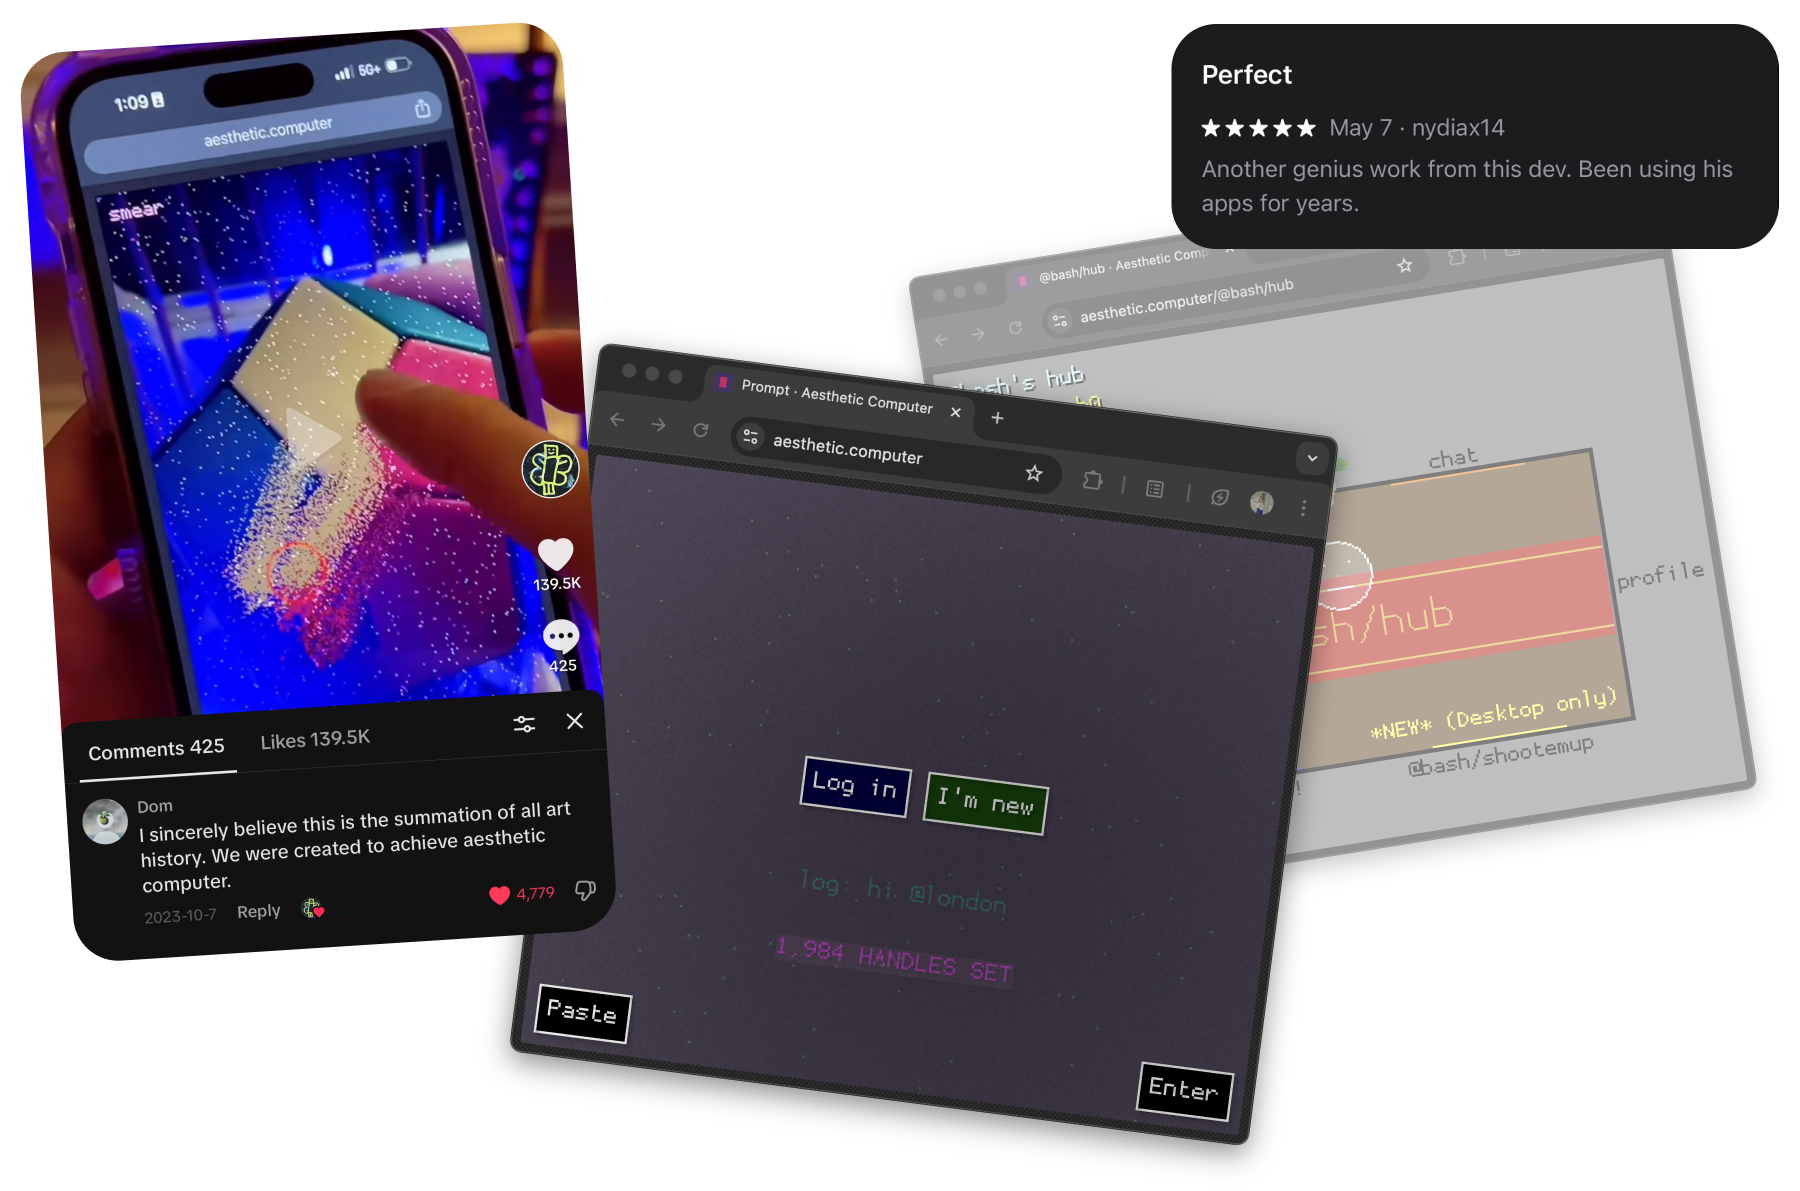
\includegraphics[width=\textwidth]{platform-screenshot}\\[4pt]
  {\small\color{acgray} \textbf{Fig.\,1} --- \ac{} running on mobile and desktop. The platform hosts 600+ interactive pieces across 2,800 registered users. Social features include chat, multiplayer, and instant QR sharing.}
\end{center}

\vspace{1em}

\begin{center}
  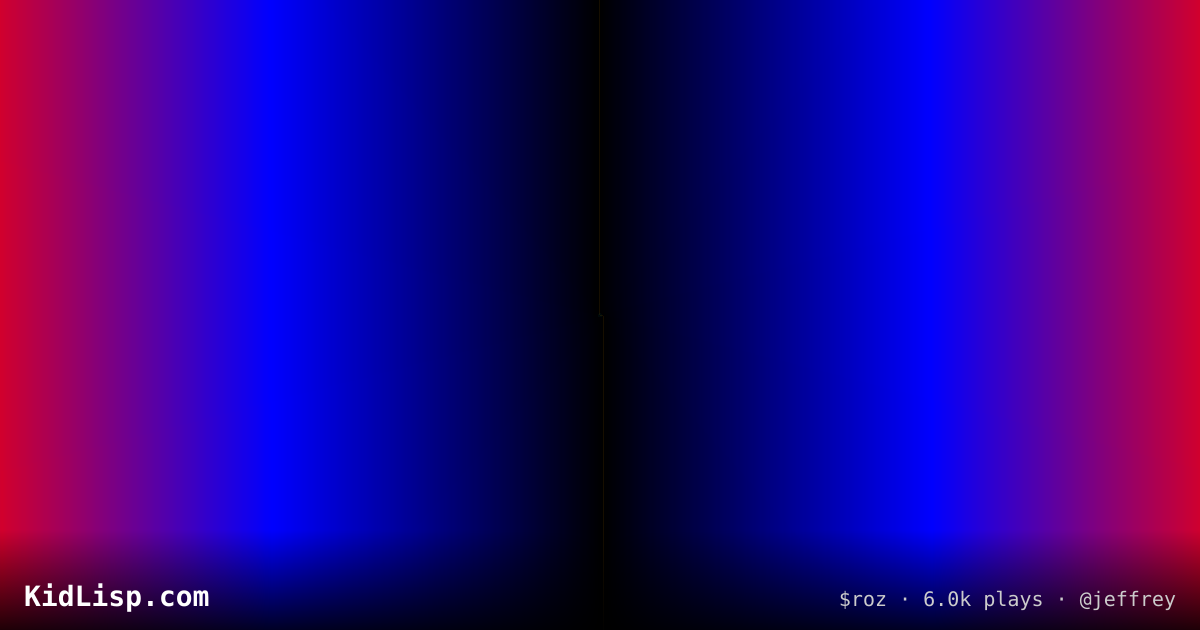
\includegraphics[width=\textwidth]{kidlisp-featured}\\[4pt]
  {\small\color{acgray} \textbf{Fig.\,2} --- \textit{\$roz} by @jeffrey, a KidLisp generative piece with 6,000+ plays. KidLisp programs run directly in the browser and on AC Native hardware. Over 16,000 programs have been written on the platform.}
\end{center}

\vspace{1em}

\begin{center}
  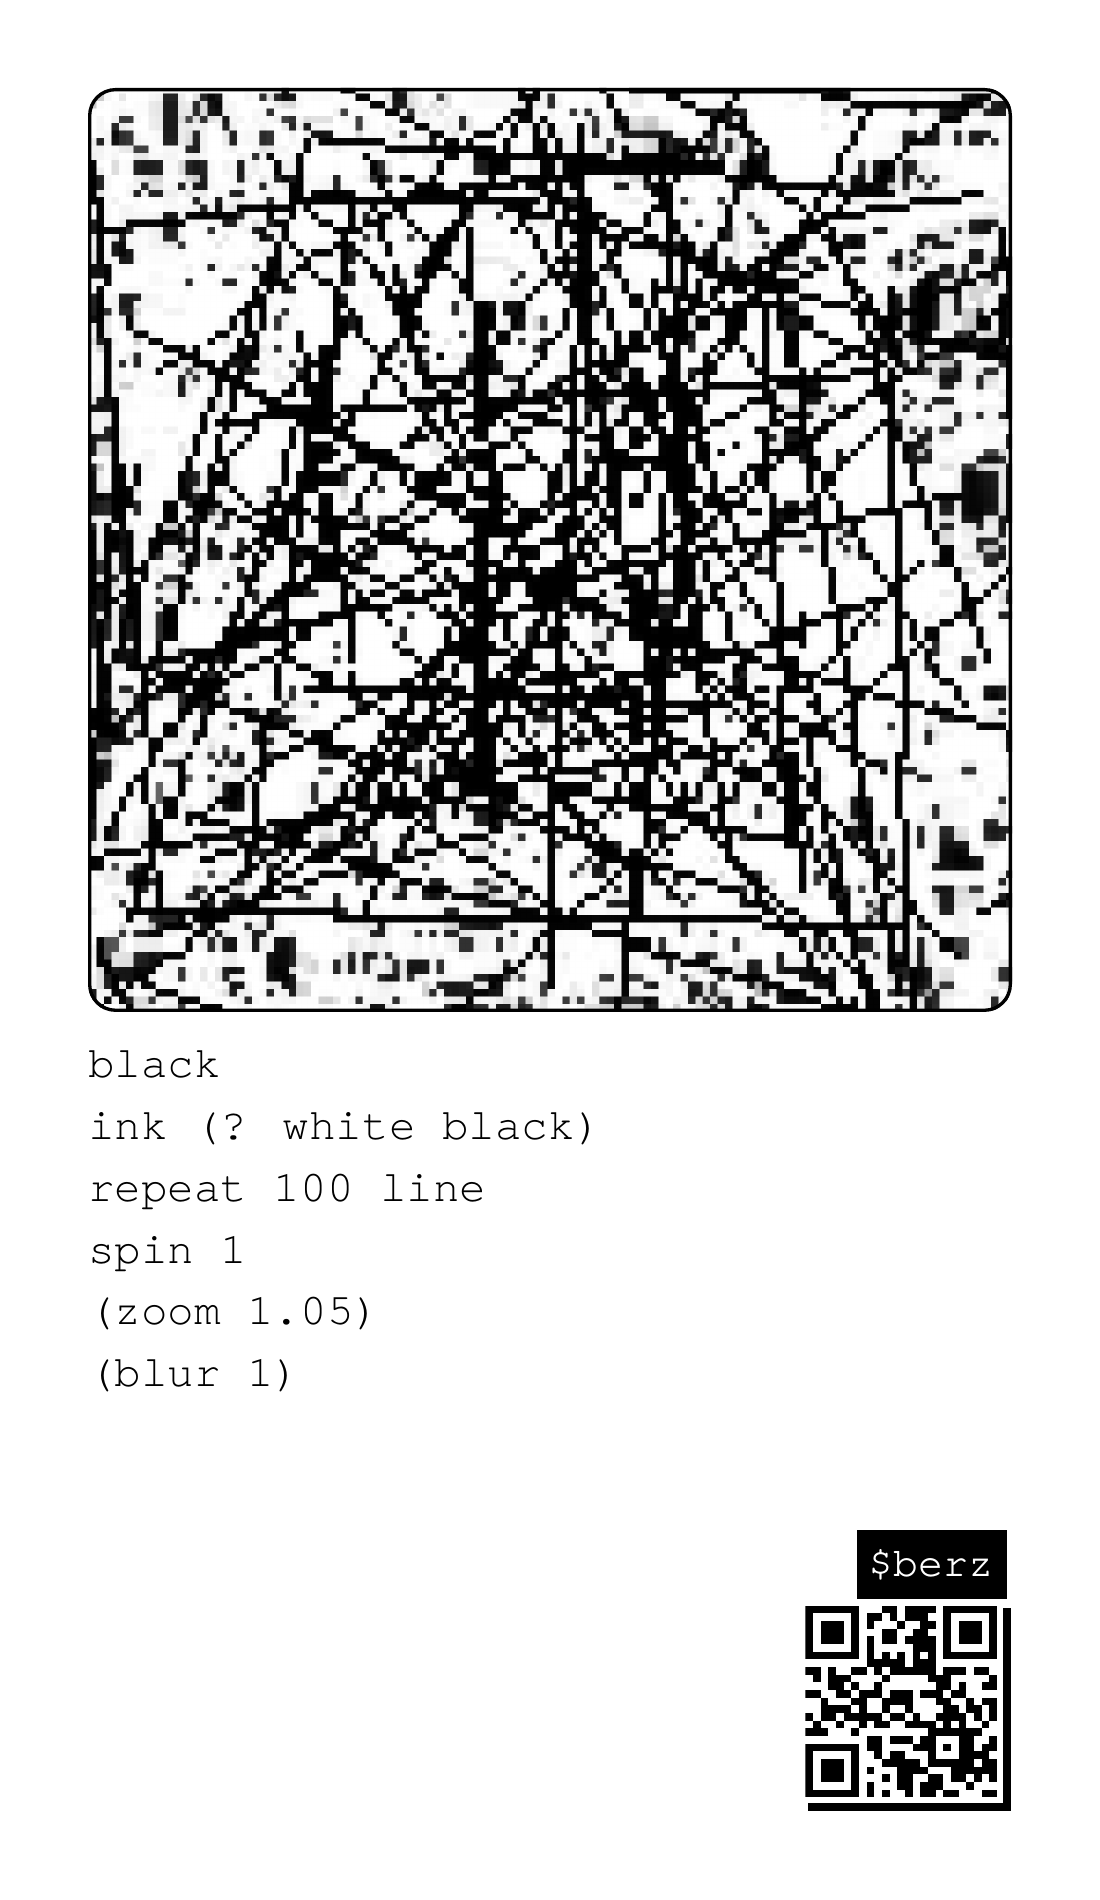
\includegraphics[height=0.285\textheight]{card-berz}\hspace{0.25em}%
  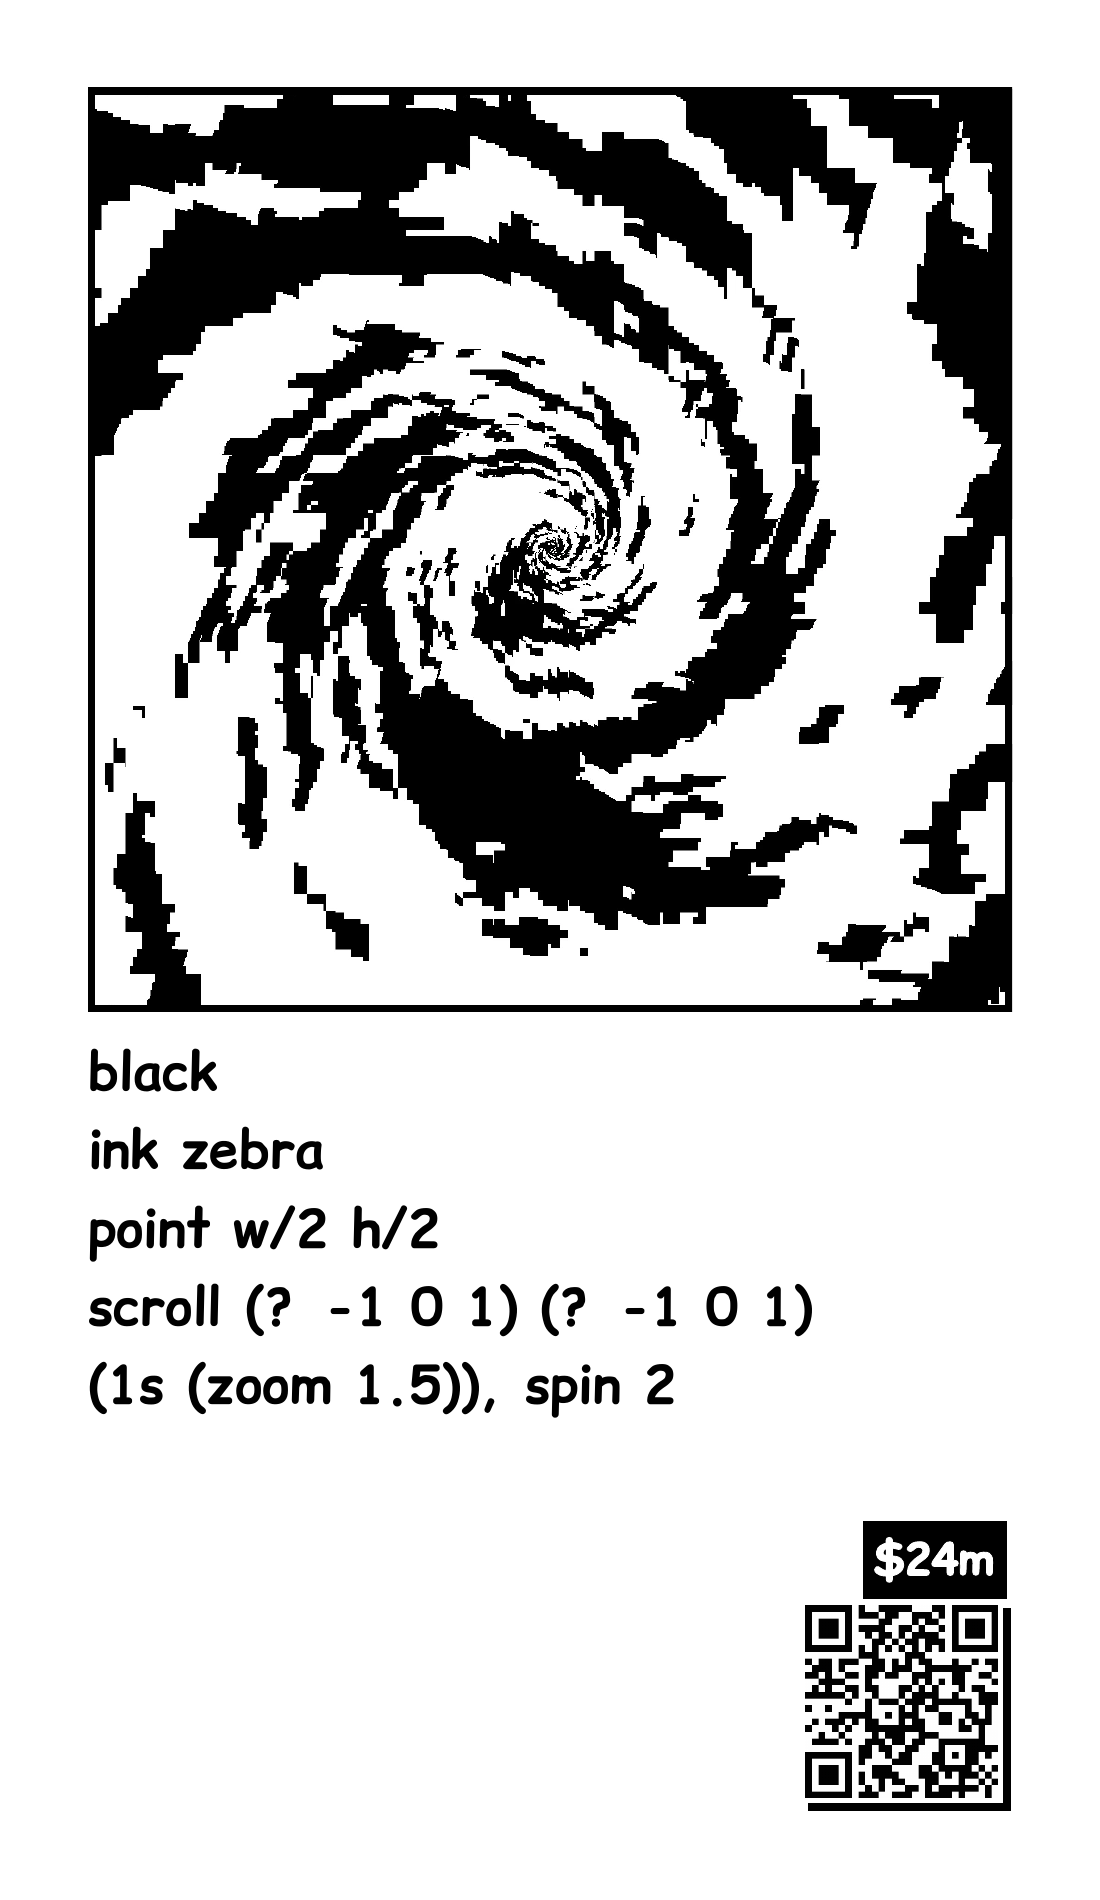
\includegraphics[height=0.285\textheight]{card-24m}\hspace{0.25em}%
  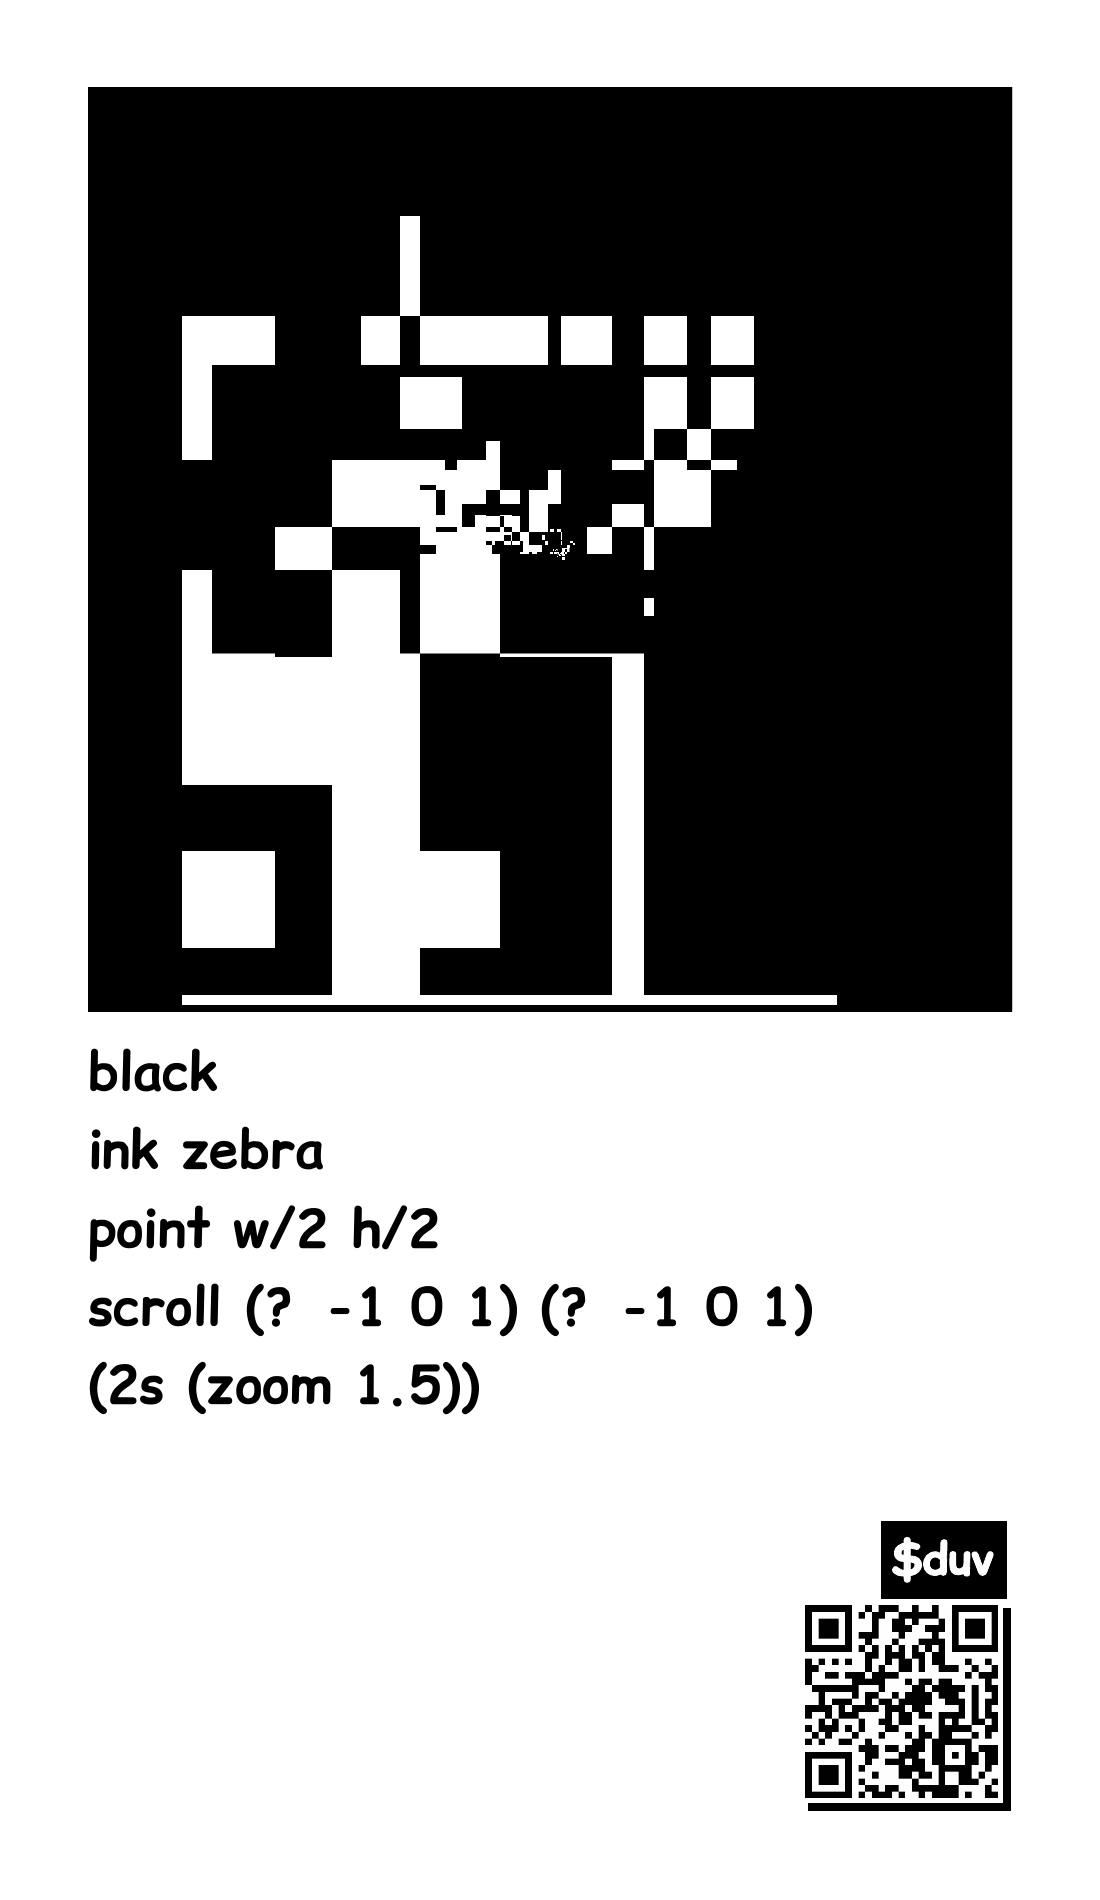
\includegraphics[height=0.285\textheight]{card-duv}\hspace{0.25em}%
  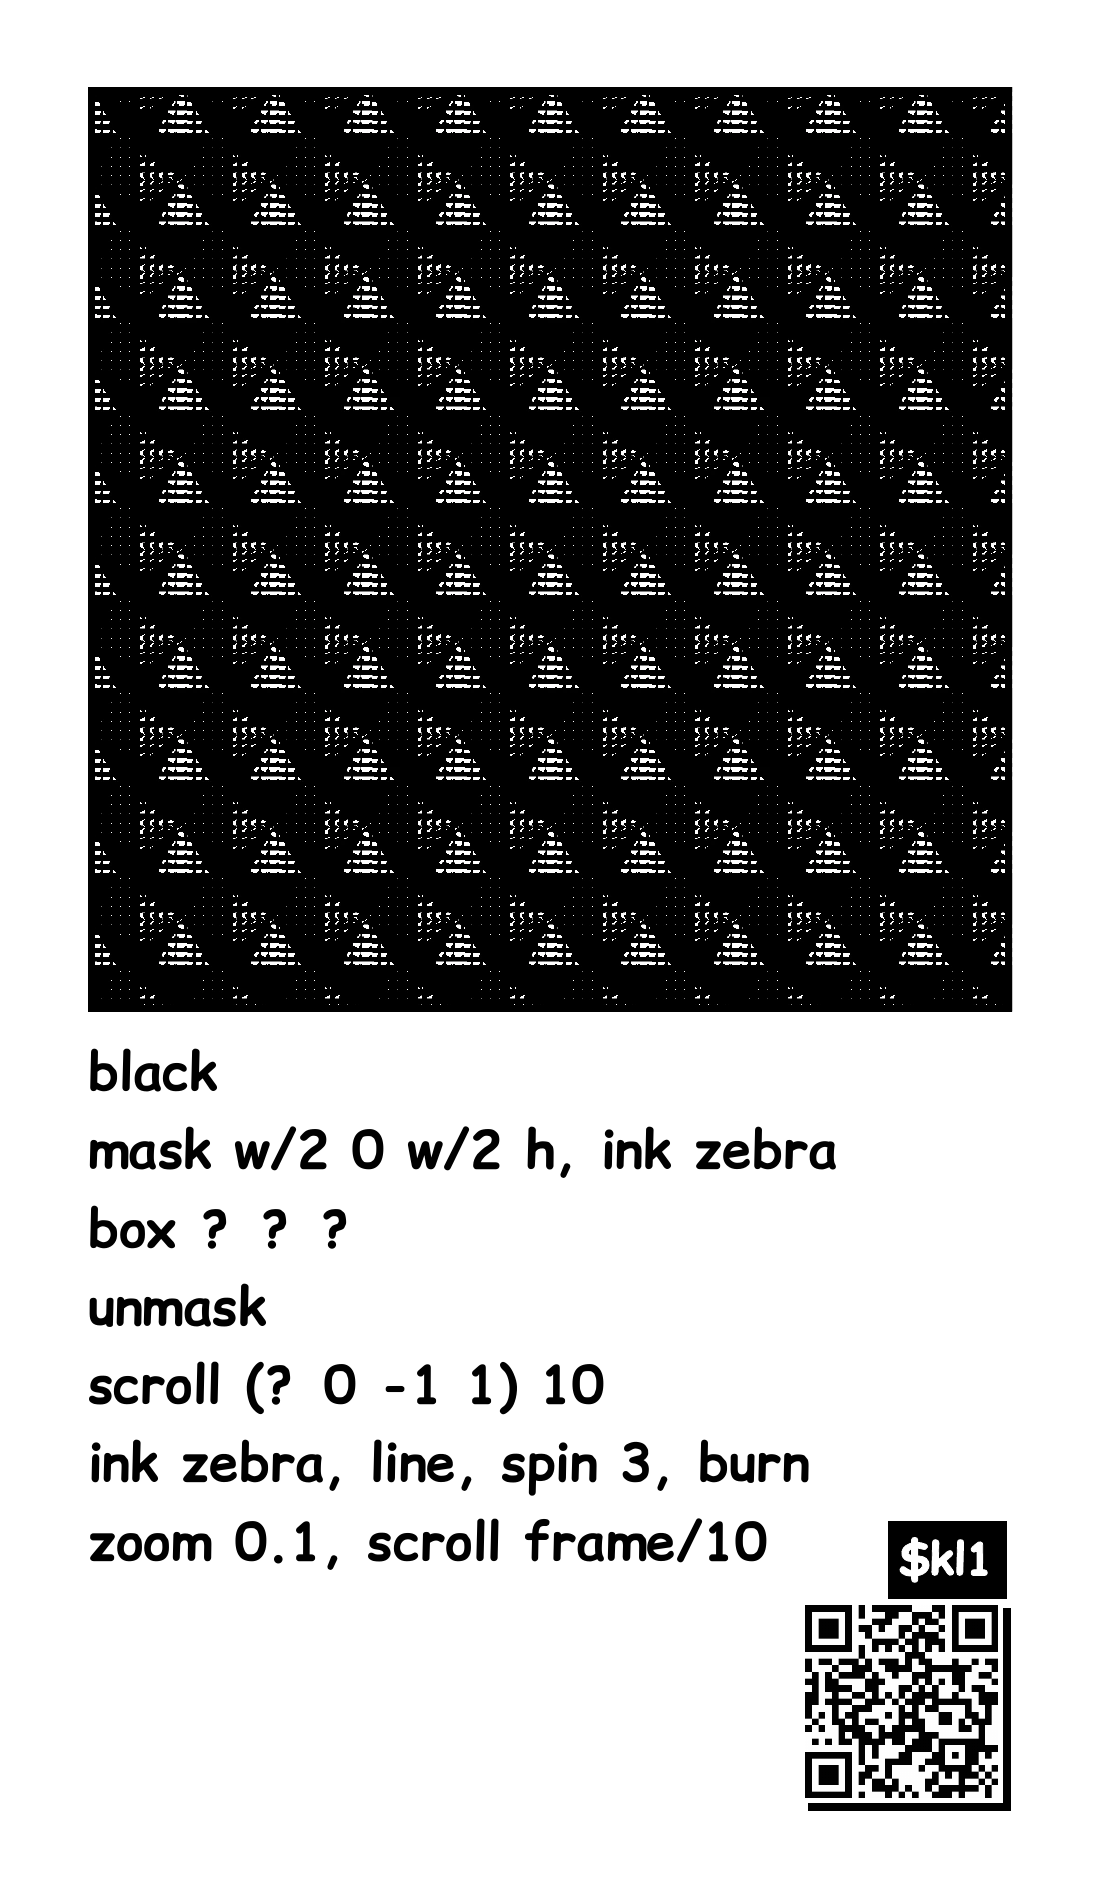
\includegraphics[height=0.285\textheight]{card-kl1}\\[6pt]
  {\small\color{acgray} \textbf{Fig.\,3} --- Four KidLisp pieces as printable cards: \textit{\$berz}, \textit{\$24m}, \textit{\$duv}, and \textit{\$kl1}. Each card is a self-contained program---the pixel image at top is the live output; the code underneath is the complete source. Printed cards were produced for Casey Reas \& Lauren Lee McCarthy's ``Social Software'' course at UCLA (2026). QR codes link back to the live piece on \ac.}
\end{center}

\vspace{1em}

\begin{center}
  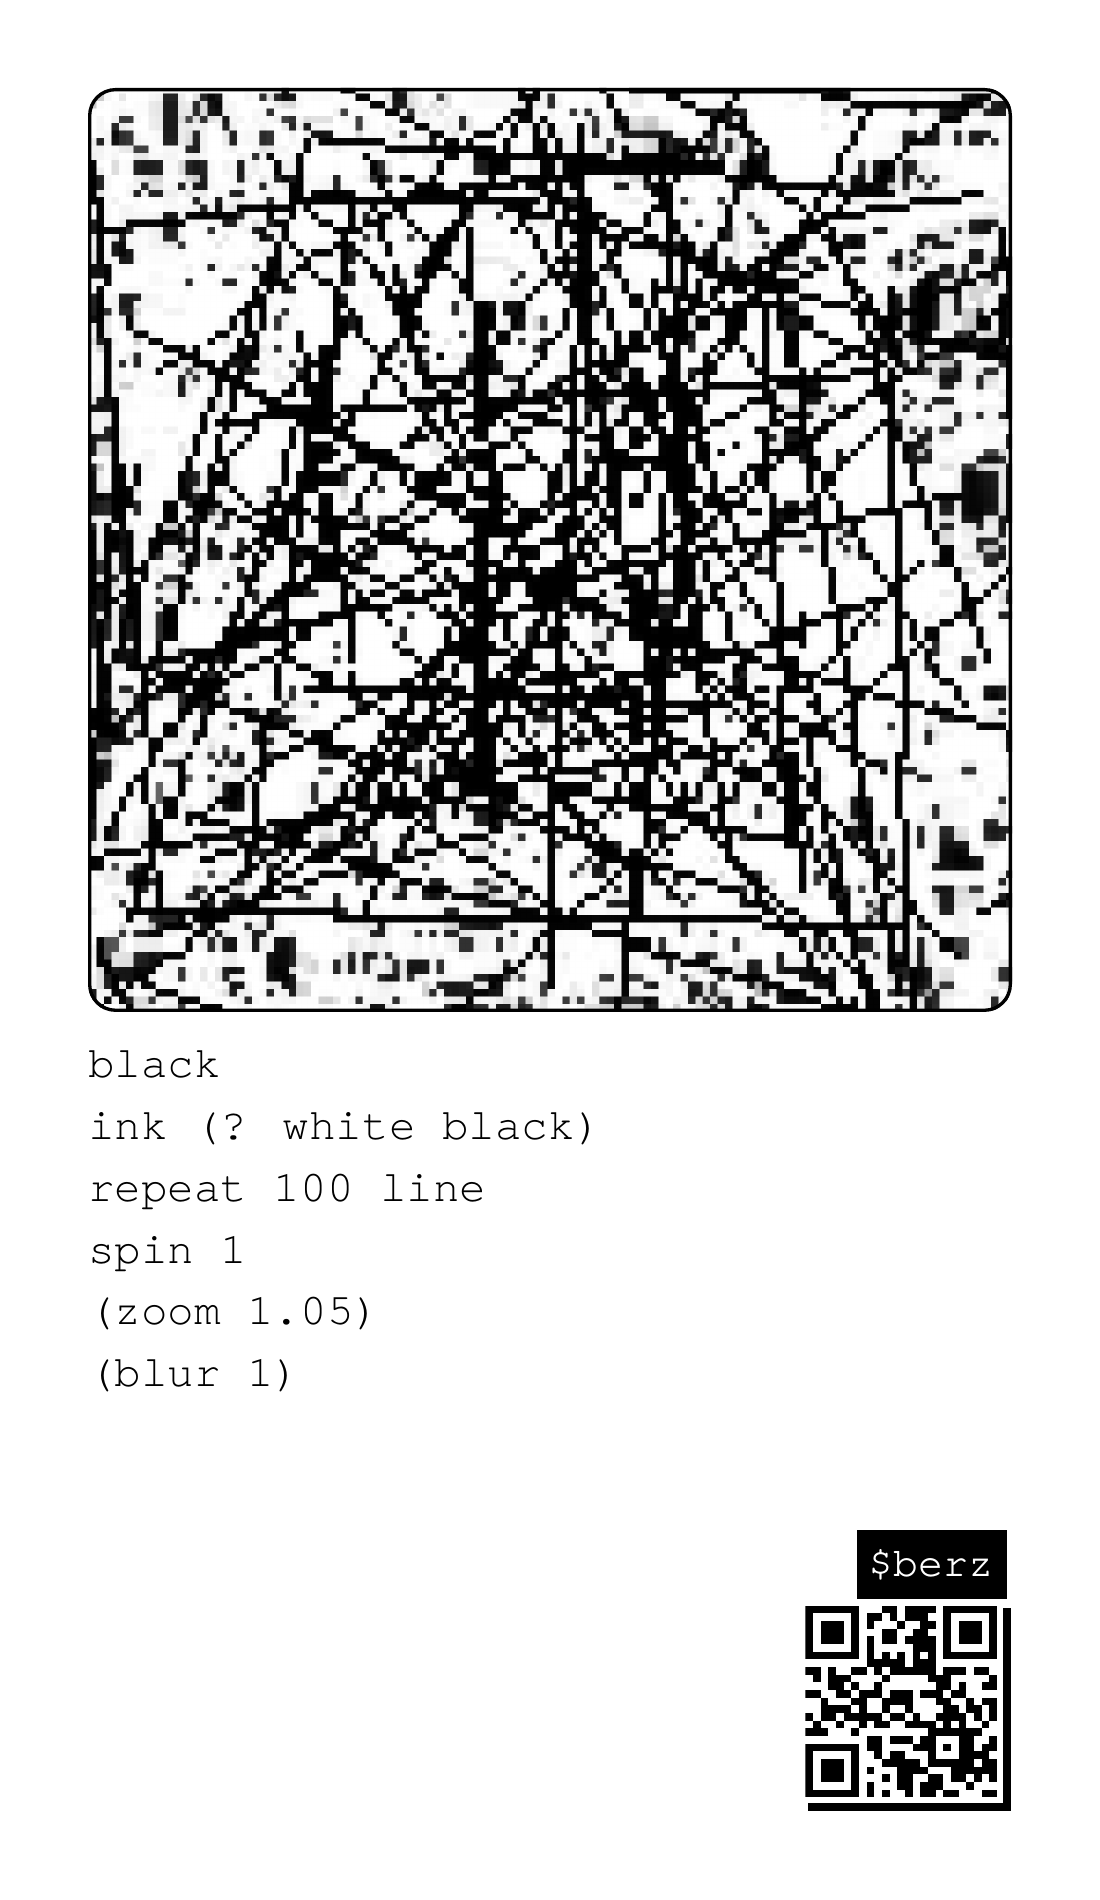
\includegraphics[width=0.42\textwidth]{card-berz}\\[4pt]
  {\small\color{acgray} \textbf{Fig.\,4} --- \textit{\$berz} up close. Six lines of KidLisp produce a recursive wire-tangle that spins, zooms, and blurs each frame. No imports, no build step, no dependencies---the entire program is visible on the card. Cards are 2.75\,$\times$\,4.75 inches, monochrome, screen-printable.}
\end{center}

\vspace{1em}

\begin{center}
  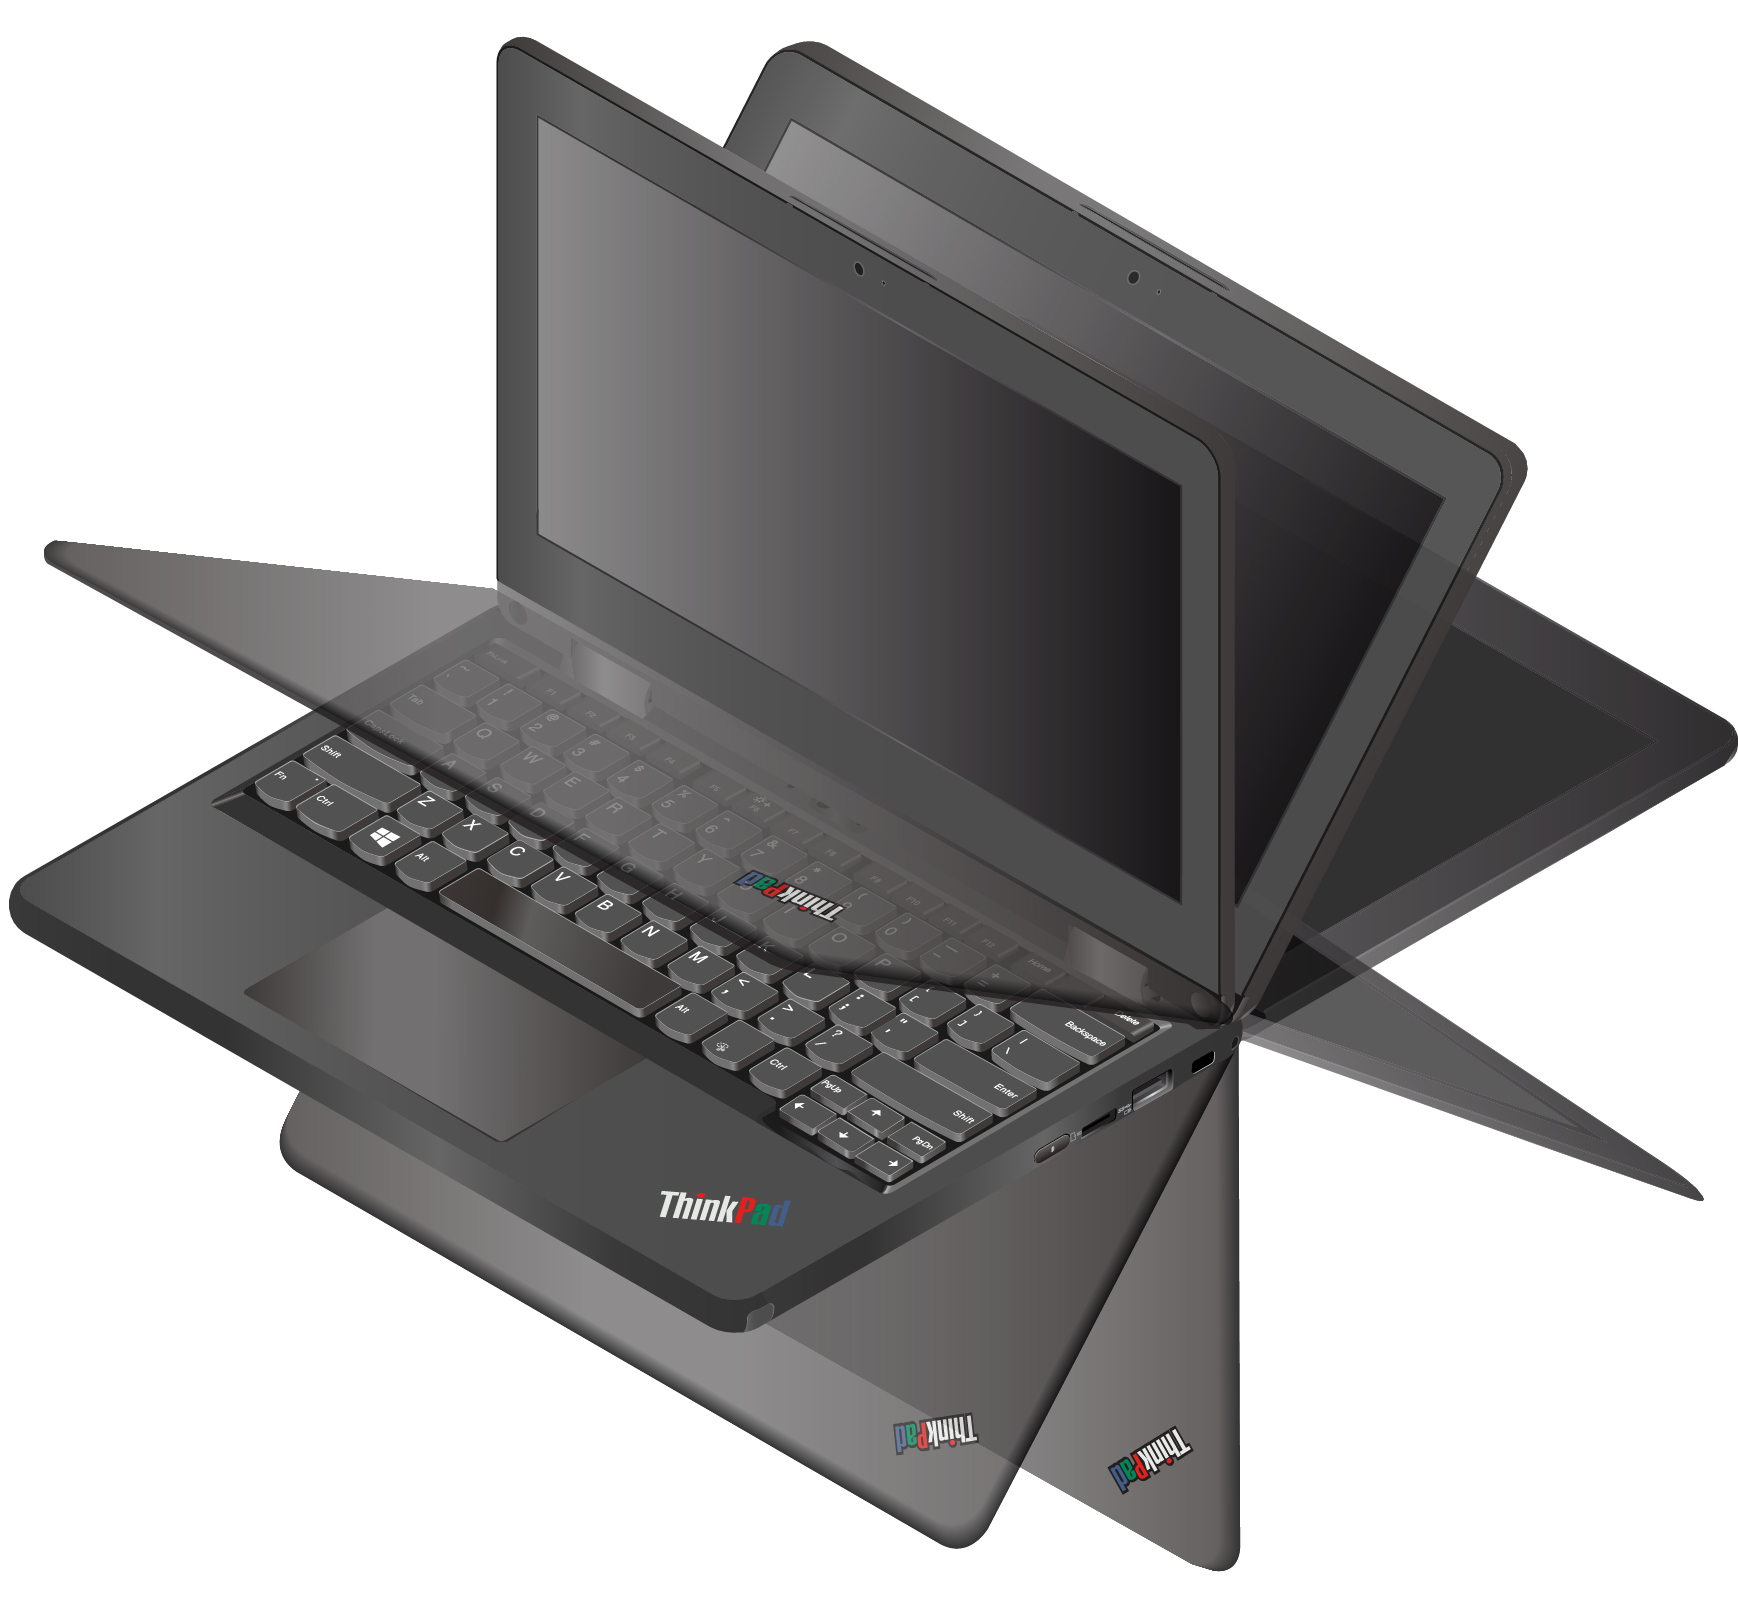
\includegraphics[width=0.7\textwidth]{hardware-yoga}\\[4pt]
  {\small\color{acgray} \textbf{Fig.\,5} --- Target hardware: a Lenovo Yoga convertible laptop. AC Native boots from USB on x86\_64 UEFI machines, turning commodity hardware into a dedicated creative instrument without replacing the factory OS.}
\end{center}

% =======================================================================
\achead{Statements}

\acsubhead{Artistic Merit}

\ac{} treats the computer itself as an unfinished instrument---a site for ongoing artistic invention rather than a fixed consumer product. By building from bare metal (custom kernel, framebuffer rendering, sample-level audio synthesis), we recover the directness that early personal computing promised but commercial platforms abandoned. The work sits at the intersection of software art, instrument design, and language design: KidLisp is simultaneously a tool and a medium, and AC Native transforms commodity laptops into dedicated creative instruments. The artistic claim is that how we build computers is itself a creative act with cultural consequences.

\acsubhead{Technology and Culture}

Consumer operating systems have become attention-extraction machines---optimized for engagement metrics, not creative agency. AC Native offers a counter-model: a computer that boots directly into a single piece of art software and does nothing else. This is not nostalgia for early computing but a forward-looking argument that the personal computer's design is a cultural question, not a settled technical one. KidLisp extends this argument to programming itself---demonstrating that a language can be designed for artistic expression rather than industrial production. The 16,000+ programs written in KidLisp suggest this resonates beyond our own practice.

\acsubhead{Public Engagement}

We propose three forms of public engagement. First, hands-on KidLisp workshops at LACMA where participants write generative art programs that run on AC Native hardware---no prior coding experience required. Second, an installation of multiple AC Native stations where visitors experience creative computing as a direct, instrument-like interaction. Third, open ``build days'' where we assemble USB drives and document the process publicly, inviting visitors into the making of the system itself. All curricula, documentation, and software will be published openly for other artists and institutions to adopt.

% =======================================================================
\achead{Timeline}

This proposal aligns to the Lab's new biennial calendar: a working-prototype milestone at the \textbf{2027 Symposium} and a completed public premiere at the \textbf{2028 Demo Day}. The cohort structure (3--5 recipients plus invitational projects) is well-suited to this work---AC Native's USB-bootable format means other cohort artists can bring their own pieces to the system, and we can cross-pollinate at Symposium without waiting for Demo Day. Two recent Lab projects sit directly in our neighborhood: Casey Reas's 2023 \textit{METAVASARELY and An Empty Room} (generative systems) and Lauren Lee McCarthy's 2022 \textit{Auto} (public/social interface design). Reas and McCarthy co-teach UCLA's Social Software course, which I am an Author in Residence in during this application year---their class is where the KidLisp cards shown in Fig.\,3 were first printed and circulated.

\renewcommand{\arraystretch}{1.4}
\begin{tabularx}{\textwidth}{@{}lX@{}}
  \textbf{Fall 2026 -- Spring 2027} & \textbf{Hardware \& Curriculum}---Expand AC Native compatibility to 5+ laptop models; build multi-piece boot menu; design the 3-level KidLisp workshop curriculum; produce printed reference cards (extending the sosoft card template used at UCLA). \\
  \textbf{Spring -- Summer 2027} & \textbf{Pre-Symposium: First Workshops}---Run 2 pilot workshops at LACMA; assemble the first prototype multi-station installation; publish v0 of the open-source build guide. \\
  \textbf{Fall 2027} & \textbf{2027 Symposium (works-in-development)}---Live AC Native demonstration: visitors (and cohort artists) boot the OS on their own laptops from a USB stick. Public KidLisp workshop in the museum. Talk / in-conversation on generative computing, situated alongside the 2023 cohort's work. \\
  \textbf{Winter 2027 -- Summer 2028} & \textbf{Full Installation + Extended Workshops}---Kiosk-mode hardening; 20+ bootable USB drives for visitor take-home; 4 additional workshops; complete documentation; translate workshop curriculum (English + Spanish, matching AC's existing translation pipeline). \\
  \textbf{Fall 2028} & \textbf{2028 Demo Day (completed project)}---Public premiere of the multi-station AC Native installation in the LACMA galleries. Open-source v1.0 release with full build pipeline, hardware compatibility matrix, and workshop curriculum available for other institutions to adopt. Public programs introducing the system to teachers, museum educators, and other artists. \\
\end{tabularx}
\renewcommand{\arraystretch}{1.0}

% =======================================================================
\achead{Budget}

\renewcommand{\arraystretch}{1.3}
\begin{tabularx}{\textwidth}{@{}Xr@{}}
  Artist fee (24 months, Fall 2026 -- Fall 2028) & \$22,000 \\
  Studio hardware (dev machines, displays) & \$3,500 \\
  Installation laptops (5 × \$400 refurbished) & \$2,000 \\
  NuPhy analog keyboards for installation (5 × \$120) & \$600 \\
  USB drives, cables, peripherals & \$500 \\
  Installation fabrication (furniture, mounts) & \$2,500 \\
  Workshop materials (printed guides, KidLisp reference cards) & \$1,200 \\
  \textbf{2027 Symposium contribution} (travel, cohort demo USB kit, on-site demo station) & \$2,500 \\
  \textbf{2028 Demo Day premiere} (install setup, public-program support) & \$3,000 \\
  Server + compute infrastructure (hosting, CDN, CI/CD) & \$3,500 \\
  Documentation production (video, photography, translation) & \$2,000 \\
  Contingency (10\%) & \$3,700 \\
  {\color{acgray}\hrulefill} & {\color{acgray}\hrulefill} \\[-0.3em]
  \textbf{Total Requested} & \textbf{\$47,000} \\
\end{tabularx}
\renewcommand{\arraystretch}{1.0}

\vspace{0.2em}
{\color{acgray} Other funding: open-source sponsorship via GitHub Sponsors and Liberapay supplements ongoing infrastructure costs (hosting, domains, CI).}

% =======================================================================
% CV
% =======================================================================

\achead{Curriculum Vitae}

\begin{center}
  {\color{acgray} Jeffrey Alan Scudder · \href{https://aesthetic.computer}{aesthetic.computer} · Los Angeles, CA}
\end{center}

Jeffrey Alan Scudder (b.\,1989, Assonet, MA) is an artist based in Los Angeles, working across stretched canvas, custom software, and live performance. Yale School of Art MFA (2013). He is the creator of \ac{}, Whistlegraph, and No Paint; his open-source tools \textit{No Paint} (2020) and \textit{notepat} (2024) each reached the front page of Hacker News. Work is held in the collections of KADIST (San Francisco) and SMK---National Gallery of Denmark. He is currently Author in Residence at UCLA, working with Casey Reas, and hosts biweekly NELA Computer Club demos at Plot.Place in Chinatown, Los Angeles.

\acsubhead{Education}

\cvline{2013}{Yale School of Art---MFA (Sculpture)}
\cvline{2011}{Ringling College of Art + Design---BFA (Fine Art)}
\cvline{2010}{AICAD New York Studio Program Residency}

\vspace{0.3em}
\begin{minipage}[t]{0.47\textwidth}
\acsubhead{Residencies}
\cvline{2026}{Author in Residence, UCLA (Casey Reas)}
\cvline{2019}{Internet Archive Artist in Residence}
\cvline{2018}{Gazell.io Art House Web Residency}
\cvline{2017}{Schloss-Post Web Residencies (ZKM)}
\end{minipage}%
\hfill
\begin{minipage}[t]{0.47\textwidth}
\acsubhead{Teaching}
\cvline{2026}{Author in Residence, UCLA (Casey Reas)}
\cvline{2024}{UCLA DMA Summer: Interactivity}
\cvline{2019}{Asst.\ Professor, Southern Oregon U.}
\cvline{2016}{Visiting Professor, UCLA DMA}
\cvline{13--16}{Adjunct Professor, Parsons}
\end{minipage}

\acsubhead{Selected Solo Exhibitions}

\cvline{2022}{Ten Whistlegraphs, Feral File (w/ Whistlegraph)}
\cvline{2018}{Radical Digital Painting: LA, The Newsstand Project \& CAP}
\cvline{2017}{Tumpin, left.gallery (Online)}
\cvline{2017}{Imaginary Screenshots, Whitcher Projects, Los Angeles}
\cvline{2016}{No Paint: Release One, Essex Flowers (Digital Commission)}

\acsubhead{Selected Group Exhibitions}

\cvline{2026}{47th Venice Family Clinic Art Exhibition + Auction, Venice, CA}
\cvline{2025}{Turbo Cheap (inaugural exhibition), Los Angeles}
\cvline{2019}{Internet Archive Artist in Residency Exhibition}
\cvline{2018}{OPEN CODES (Schloss Solitude Web Residencies), ZKM, Karlsruhe}
\cvline{2018}{Radical Digital Painting w/ Julia Yerger, Johannes Vogt Gallery, NYC}
\cvline{2018}{Make Pictures (curated), bitforms gallery, NYC}
\cvline{2015}{P.S.1 Commencement, ALLGOLD @ MoMA PS1 Printshop, LIC, NY}
\cvline{2013}{Apartment Show (hosted by Nouriel Roubini), NYC}
\cvline{2009}{The New Easy, Artnews Projects, Berlin}

\acsubhead{Selected Lectures \& Performances {\normalfont\color{acgray}(65+ total)}}

\cvline{2026}{NELA Computer Club demos (biweekly), Plot.Place, Chinatown, LA}
\cvline{2022}{The Longest Whistlegraph Ever (so far), New Museum, NYC}
\cvline{2020}{New Dynamic Graphics: Whistlegraph Recital, Korea HCI (keynote)}
\cvline{2019}{New Dynamic Graphics, India HCI 19 (keynote), Hyderabad}
\cvline{2019}{RDP @ RAFLOST Festival, Iceland}
\cvline{2018}{RDP, 35c3: Chaos Communication Congress, Leipzig}
\cvline{2018}{Casey Reas \& JAS in Conversation, bitforms gallery, NYC}
\cvline{2018}{RDP @ 1st Annual HASH Award, ZKM, Karlsruhe}
\cvline{2018}{RDP @ Pioneer Works, Brooklyn, NY}
\cvline{2018}{European tour (15+ venues) w/ Goodiepal \& Pals}
\cvline{2017}{Northeast US Lecture Tour (Parsons, Harvard, Yale, RISD, Temple, Rutgers)}
\cvline{2017}{RDP @ Cafe OTO, London \& Neumeister Bar-Am, Berlin}

\acsubhead{Collections}

KADIST Foundation, San Francisco\\
SMK---National Gallery of Denmark, Copenhagen

\acsubhead{Selected Press \& Writing}

\cvline{2024}{\textit{notepat}, Hacker News (front page)}
\cvline{2023}{Whistlegraph---A new audience for generative art, \textit{Dirt}}
\cvline{2023}{Sex: The Whistlegraph Zine, \textit{Sex Magazine}}
\cvline{2020}{No Paint, Hacker News (front page)}
\cvline{2019}{Drawing is the best videogame, \textit{The Creative Independent}}
\cvline{2018}{Radical Digital Painting \& Political Rock, \textit{Are.na Blog}}
\cvline{2018}{\textit{Harvard Advocate}, Winter 2018 (Noise)}
\cvline{2017}{Artist Profile: Jeffrey Alan Scudder, \textit{Rhizome}}
\cvline{2017}{A Manifesto for Radical Digital Painting, \textit{Schlosspost}}
\cvline{2017}{Microsoft Paint's Influence on Artists Is Bigger Than You Might Think, \textit{Artsy}}

\acsubhead{Software \& Platforms}

\cvline{2021--}{\ac{}---creative computing platform (\href{https://aesthetic.computer}{aesthetic.computer})}
\cvline{2025--}{AC Native---bare-metal creative computing OS (USB-bootable Linux)}
\cvline{2024--}{KidLisp---programming language for generative art (16,000+ programs)}
\cvline{2024--}{\textit{notepat}---polyphonic synthesizer instrument (8,466 lines)}
\cvline{2016--}{No Paint---radical paint program (\href{https://nopaint.art}{nopaint.art})}
\cvline{2016--}{Whistlegraph---collaborative performance software (w/ Camille Klein \& Alex Freundlich)}

\vfill
\begin{center}
  \color{acgray}
  \href{https://aesthetic.computer}{aesthetic.computer}\enspace·\enspace
  \href{mailto:mail@aesthetic.computer}{mail@aesthetic.computer}\enspace·\enspace
  LACMA Art + Technology Lab 2026
\end{center}

% =======================================================================
% APPENDIX: Original Call for Proposals
% =======================================================================
\newpage
\achead{Appendix: LACMA 2026 Call for Proposals}

\begin{center}
  {\color{acgray}\small Source: \href{https://www.lacma.org/art/lab/grants}{lacma.org/art/lab/grants} · Retrieved April 2026}
\end{center}

\vspace{0.5em}

The Los Angeles County Museum of Art invites artists worldwide to apply for Art + Technology Lab grants. The initiative supports a ``safe-to-fail rapid prototyping environment'' where creators explore intersections of art, science, and emerging technology. The program emphasizes experimentation over finished products.

\acsubhead{Key Details}

\begin{tabularx}{\textwidth}{@{}lX@{}}
  \textbf{Deadline} & April 22, 2026, 11:59\,PM PST \\
  \textbf{Notification} & July 2026 \\
  \textbf{Project Start} & As early as fall 2026 \\
  \textbf{Grant Amount} & Up to \$50,000 per project \\
  \textbf{Duration} & Typically two years \\
  \textbf{Selected} & 3--5 via open call, plus up to 2 invitational \\
\end{tabularx}

\acsubhead{Eligibility}

Artists and collectives worldwide may apply. Prior technological experience is not required. Applicants need not be Los Angeles--based.

\acsubhead{Support Provided}

Financial grants cover artist fees and direct costs including materials. Recipients also receive in-kind support: mentorship, coaching, and access to partner technologies from Hyundai Motor, Snap Inc., Anthropic, and academic institutions including MIT Media Lab Space Exploration Initiative and NASA Jet Propulsion Laboratory.

\acsubhead{Evaluation Criteria}

Projects must demonstrate:
\begin{itemize}
  \item Artistic merit and artist-led vision
  \item Exploration of emerging technology
  \item Models or methods valuable to broader communities
  \item Public engagement opportunities during development
\end{itemize}

\acsubhead{Application Requirements}

\begin{itemize}
  \item Project name and three descriptive words
  \item One-sentence description
  \item Full project description (500-word maximum)
  \item Artist biography / CV
  \item Artistic merit statement (100 words max)
  \item Discussion of technology--culture dialogue (100 words max)
  \item Public engagement plan (100 words max)
  \item Funding sources and conditions
  \item Detailed budget with milestones
  \item Up to 5 images / renderings (JPEG format)
  \item Video links (under 5 minutes)
\end{itemize}

\vfill
\begin{center}
  \color{acgray}
  Apply: \href{https://lacma.submittable.com/submit/348727/2026-art-technology-lab-grants}{lacma.submittable.com}
\end{center}

\end{document}
